	\chapter*{Anexo 1 PCB} % si no queremos que añada la palabra "Capitulo"
	\addcontentsline{toc}{chapter}{Anexo 1} % si queremos que aparezca en el índice
	\markboth{Anexo 1}{Anexo 1} % encabezado
	
		Para el dise\~no de la placa PCB se usó la herramienta software de código abierto KiCad, plataforma para la creación y dise\~no de esquemáticos de circuitos electrónicos y sus correspondientes archivos de fabricación de placas de circuito impreso. El hecho de ser una plataforma de código abierto lo hace perfecto para proyectos orientados a la creación de hardware electrónico.
		
		Kicad no tiene limitación del tama\~no de la placa y puede manejar facilmente hasta 16 capas de cobre y hasta 12 capas técnicas. Puede generar todos los ficheros necesarios para la fabricación de placas de circuito impreso, tales como: Gerber files, component locantion files...
		
		Podemos descargar KiCad desde http://www.kicad-pcb.org, donde se nos descargará un ejecutable que instalará en la ruta deseada las herramientas de KiCad.
		
		Una vez ha sido instalado KiCad, lo primero que debemos realizar es dise\~nar el Esquemático de nuestro proyecto. Para ello detallaré a continuación los pasos que seguí y el restultado que obtuve.
		
		Los pasos seguidos fueron los siguientes:
		
		\begin{itemize}	
			
			\item Lo primero de todo es crear un nuevo proyecto y guardarlo con el nombre que deseemos.
			
			\item Una vez ha sido creado el proyecto debemos pulsar sobre EESchema para comenzar a crear el esquemático del proyecto.
			
			\item Algunos componentes se encuentran en las librerías ya instalados, otros como el de la placa Arduino lo pude descargar de Internet y posteriormente asociándolo a su footprint.
			
			\item Creados todos los componentes procedí a conectarlos con cables, incluyendo las fuentes de alimentación, las tierras y definir sin conexión los pines que no utilizaré.
			
			\item Una vez el esquemático ha sido terminado hay que proceder a enlazar todos los componente del esquemático con Cvpcb.
			
		\end{itemize}
		
		El esquemático desarrollado es el siguiente:
	
		\begin{figure}[h]
			\centering
			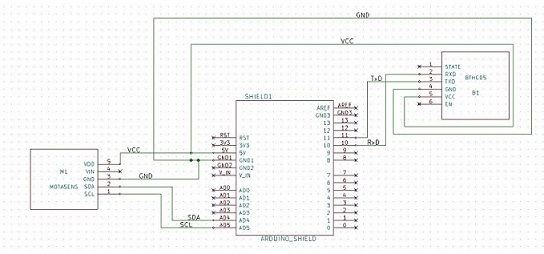
\includegraphics{imagenes/EsquematicoPCB.jpg}
			\caption{Esquemático dise\~no PCB}
			\label{contexto:figura}
		\end{figure}
		
		Ahora podemos usar la herramienta PCBnew, en la cual dise\~naremos el boceto de nuestra PCB final.
		
		Los pasos a seguir son los siguientes:
		
		\begin{itemize}	
			
			\item En primer lugar debemos fijar el tama\~no de la página a A4 y tutularla con el nombre de nuestra PCB.
			
			\item En segundo lugar debemos fijar el tamaño el clearance, ancho de las vías, separación mínima de las vías, etc.
			
			\item Accedemos al NetList, para exarminarlo y leer el Netlist actual para cargar todos los footprints asociados.
			
			\item Una vez han sido cargados, debemos colocarlos de una forma ordenada, teniendo en cuenta donde vamos a ubicar cada componente y que no haya posibles cruces de pistas ya que solo vamos a imprimir la placa a una sola capa.
			
			\item Con ''Edge Cuts'' fijaremos el tama\~no de la placa, además escogeremos la capa F.Cu con la cual creamos las vías que conectarán todos los pines.
			
			\item El resto de la placa no usada se rellenará con la capa ''F.Cu'' con la finalidad de  ser el plano de masa que irá unido a los pines tierra. Debemos dejar un espacio sin rellenar, que será donde estará la antena del dispositivo bluetooth, para evitar que se apantalle y se reduzca de forma considerable el alcance de dicha antena.
			
			\item Una vez ha sido creado y unido todo debemos realizar un chequeo de la PCB dise\~nada, lo que en nuestra herramienta se reconoce como ''Comenzar DRC''. Realizado dicho chequeo debemos comprobar que la ''Lista No Conectados'' se encuentra vacía.
			
		\end{itemize}
		
		\
		\\
		\
		
		Realizado todo esto podemos ver el resultado de la placa que hemos diseñado con PCBnew en la siguiente imagen.
		
		\begin{figure}[h]
			\centering
			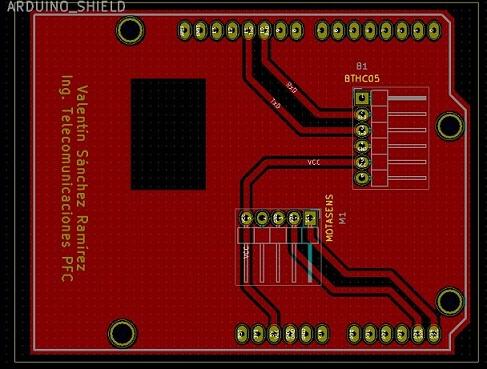
\includegraphics{imagenes/DisenoPCB.jpg}
			\caption{Dise\~no PCB en PCBnew}
			\label{contexto:figura}
		\end{figure}
		
		Además si lo deseamos podemos ver el resultado en 3D, accediendo a la pesta\~na Ver y pinchando sobre Visualización 3D. Obteniendo el siguiente resultado.
		
		\begin{figure}[h]
			\centering
			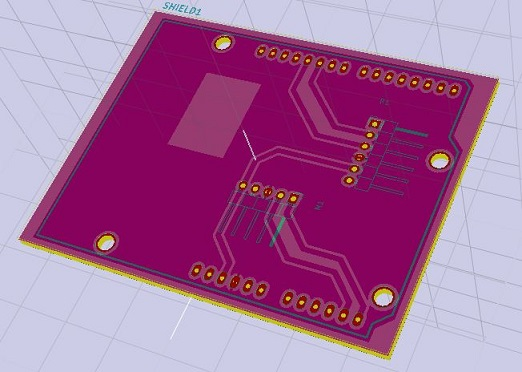
\includegraphics{imagenes/3D.jpg}
			\caption{Modelo 3D PCB}
			\label{contexto:figura}
		\end{figure}
		
		Además se nos ofrece la posibilidad de generar los ficheros Gerbers. Si queremos generarlos debemos seguir los siguientes pasos.
		
		\begin{itemize}	
			
			\item Desde PCBnew accedemos a Archivo y despues Plot.
			
			\item Elegimos ''Gerber'' en el desplagable de ''Plot Format'' y elegimos el directorio donde deseamos guardar los archivos.
			
			\item Elegimos las capas que deseamos dibujar para una placa de una sola capa.
			
			\item Hacemos click sobre ''Trazar'' para generar los Gerbers y sobre ''Generate Drill File'' para generar el archivo de drills.
			
			\item Podemos acceder a ver los archivos generados pulsando sobre el icono del GerbView.
			
		\end{itemize}

	
	\newpage
	$\ $